\documentclass[11pt]{article}
\usepackage[T1]{fontenc}
\usepackage{fontspec}
\usepackage[utf8]{inputenc}
\usepackage{url}
\usepackage{eurosym}
\usepackage{pdfpages}
\usepackage{ulem} % to use a strikeout/strikethrough font
\usepackage{color}
\newcommand{\fs}[1]{\textcolor{red}{\sout{#1}}}
\newcommand{\f}[1]{\textcolor{blue}{#1}}
\usepackage{graphicx} % Inclure des images
\usepackage{multicol} % Multi-colonnes


\usepackage[autolanguage, np]{numprint} % écriture des virgules
\usepackage[top=3cm,right=2cm,bottom=2cm,left=2cm]{geometry}


\usepackage[autolanguage, np]{numprint} % écriture des virgules

\title{HAUM}
\author{Assemblées Générales Ordinaire \& Extraordinaire}
\date{16 Janvier 2024}

\begin{document}
\maketitle

\section*{Convocation}

Madame, Monsieur,

L'association HAUM vous convoque à ses Assemblées Générales Ordinaire \& Extraordinaire qui se tiendront le :

\begin{center}
{\Large 16 Janvier 2024 à 21h00}\\
à Le Mans Innovation, \\57 Bd Demorieux au 2\textsuperscript{ème} étage, \\72 100 Le Mans
\end{center}

En cas d'impossibilité, vous pouvez vous faire représenter si vous le souhaitez (2 procurations maximum par personne présente, Statuts, art. 6).

\newpage

\hrule
\vspace{.6cm}
\begin{center}
\Large\bfseries Assemblée Générale Ordinaire
\end{center}
\vspace{.3cm}
\hrule

\vspace{1.5cm}

\section*{Déroulement}

\begin{enumerate}
    \item Présentation de l'association
    \item Rapport moral
        \begin{enumerate}
            \item Bilan
            \item Objectifs
            \item Questions
        \end{enumerate}
    \item Rapport financier
        \begin{enumerate}
						\item En images
            \item Bilan \& Objectifs
            \item Questions
        \end{enumerate}
    \item Élection du nouveau bureau
    \item Questions diverses
\end{enumerate}

\section{Présentation de l'association}

\section{Rapport Moral}

\subsection{Vie de l'association}

Le nombre d'adhérents réaugmente régulièrement depuis la fin de l'épidémie de Covid et en
2023, le HAUM a enregistré 21 cotisations dont 2 entreprises.
Depuis Août 2022 nous utilisons HelloAsso pour permettre le paiement des cotisations en ligne.

\subsection{Bilan}

\subsubsection{Le Mans Innovation}

Suite au déménagement en 2017, le HAUM a largement investi le nouveau local. L'association dispose d'un atelier propre et d'un atelier sale. Ce dernier a bénéficié d'un grand ménage lors de l'installation d'une entreprise dans les locaux de LMI. Aujourd'hui la tenue globale est correcte mais il faut veiller à ne pas en refaire un lieu de dépot. 

Grâce à un don de l'Université du Mans, le local s'est équipé en mobilier, notamment en tables et établis et des discussions sont actuellement en cours avec Le Mans Innovation pour installer une zone de stockage sur étagères. 

Il est important de mettre en place un roulement pour le rangement du HAUM et maintenir le local dans un état utilisable.

\subsubsection{Évènements}

Depuis la dernière AG (en août 2022) , Le HAUM a participé à de nombreux évènements et proposé autant de
projets innovants présentés succinctement ci-après.

\paragraph{Teriaki 2022} Morpion 3D qui n'a malheureusement pas marché suite à un problème technique.

\paragraph{Digital ON} Octobre 2022 pour un public pas très nombreux mais curieux du projet présenté. Cet évènement a d'ailleurs permis de fiabiliser le Morpion 3D présenté en août.

\paragraph{Les 24heures du code} Le projet Vrhaum, basé sur des voitures radiocommandées modifiées et augmentées a permis aux participants de construire une interface autour de nos logiciels et se mesurer sur un circuit long d'une soixantaine de mètres. Ce sujet ambitieux avec une belle implication des membres du HAUM. Les concourants et les autres organisateurs ont apprécié aussi bien le coté technique que le coté jeu de ce sujet.

\paragraph{Teriaki 2023} Le projet HAUMogramme, une table-séquenceur circulaire permettant au public de créer de la musique en déplaçant physiquement des marqueurs, a été très bien reçu.

\paragraph{Barbecue d’automne} Moment convivial autour d'un barbecue en plein mois de novembre sous la serre d'un des membres.
%a l'abri sous la serre de notre amis Nugets, la prochaine foi on s'arrangera pour pouvoir essayer la pelleteuse 

\paragraph{Les sessions bidouille} Chaque mardi soir les portes du HAUM sont ouvertes à tout ceux et celles qui veulent bien les pousser.

\subsubsection{Projets et axes}

Il y a plusieurs projets en cours. Au niveau collectif (pour des projets qui occupent
quelques personnes) on a aujourd'hui:

\begin{description}
	\item[Photographie] Sténopé, stéréo-photographie, etc\ldots
    \item[HAUMogramme] Installation sonore (et lumineuse ?)
	\item[IdiHAUM\footnotemark]\footnotetext{Nom non définitif} Solution de contrôle d'accès
\end{description}

Les réunions "projets" qui avaient été proposées et instaurées lors de la dernière année
ont été plutôt bien suivies et utiles au début de l'exercice et ont complètement disparu
pendant l'été. Elle permettaient à tous de s'informer des projets en cours régulièrement
elle sont à relancer et pourraient êtres couplées à des annonces sur le forum.

\subsection{Matériel disponible}

Le HAUM dispose actuellement du matériel suivant (entre autres):

\begin{description}
    \item Une découpeuse laser (Pret de Le Mans Innovation)
    \item Une imprimante 3D (Pret de Le Mans Innovation)
    \item Une découpeuse vinyle Caméo (plotter de découpe)
    \item Outils pour l'électronique (dont un fer à souder acquis par le HAUM cette année)
    \item Outillage électroportatif et manuel
    \item Fraiseuse CNC 3 axes de table
    \item La majorité des projets passés
\end{description}

\subsection{Objectifs}

\section{Rapport financier}

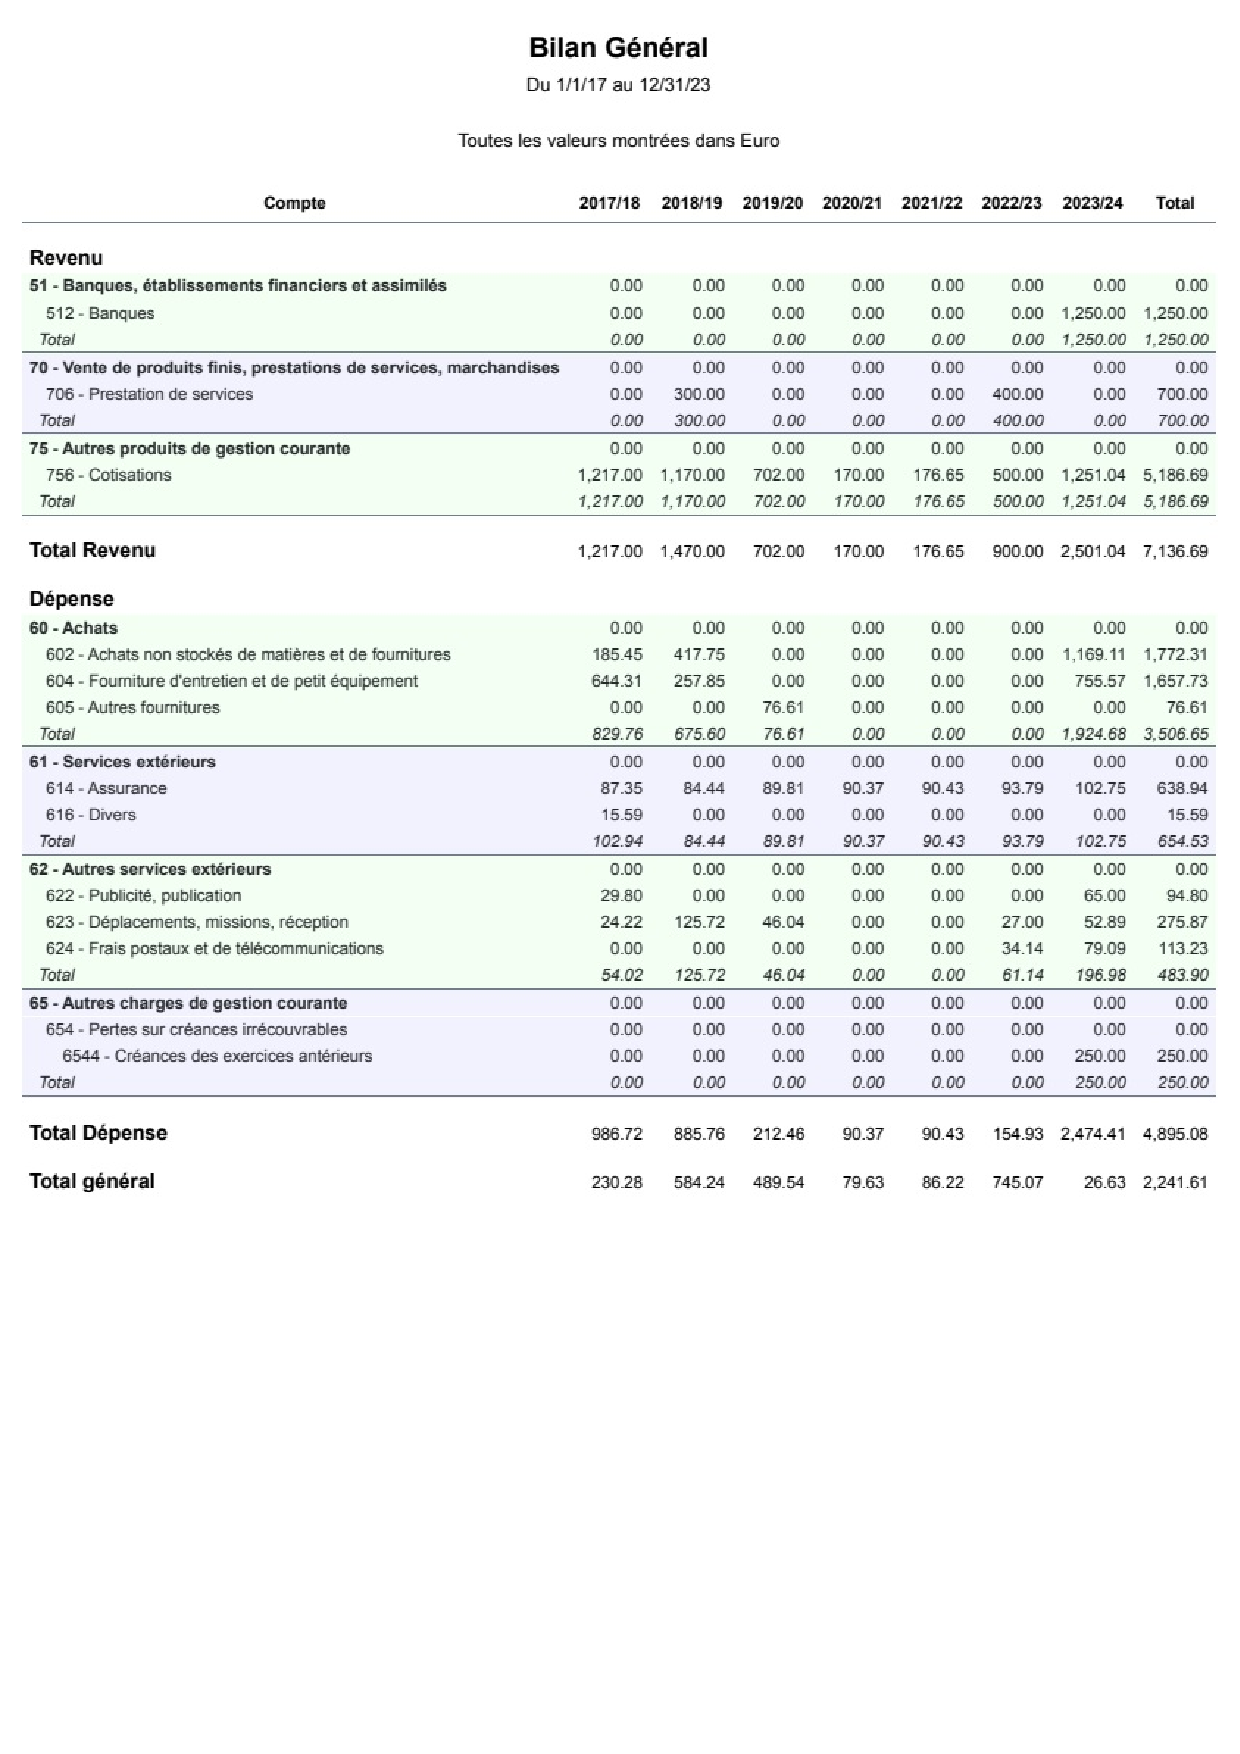
\includepdf[pages=-]{bilan2023_general.pdf}
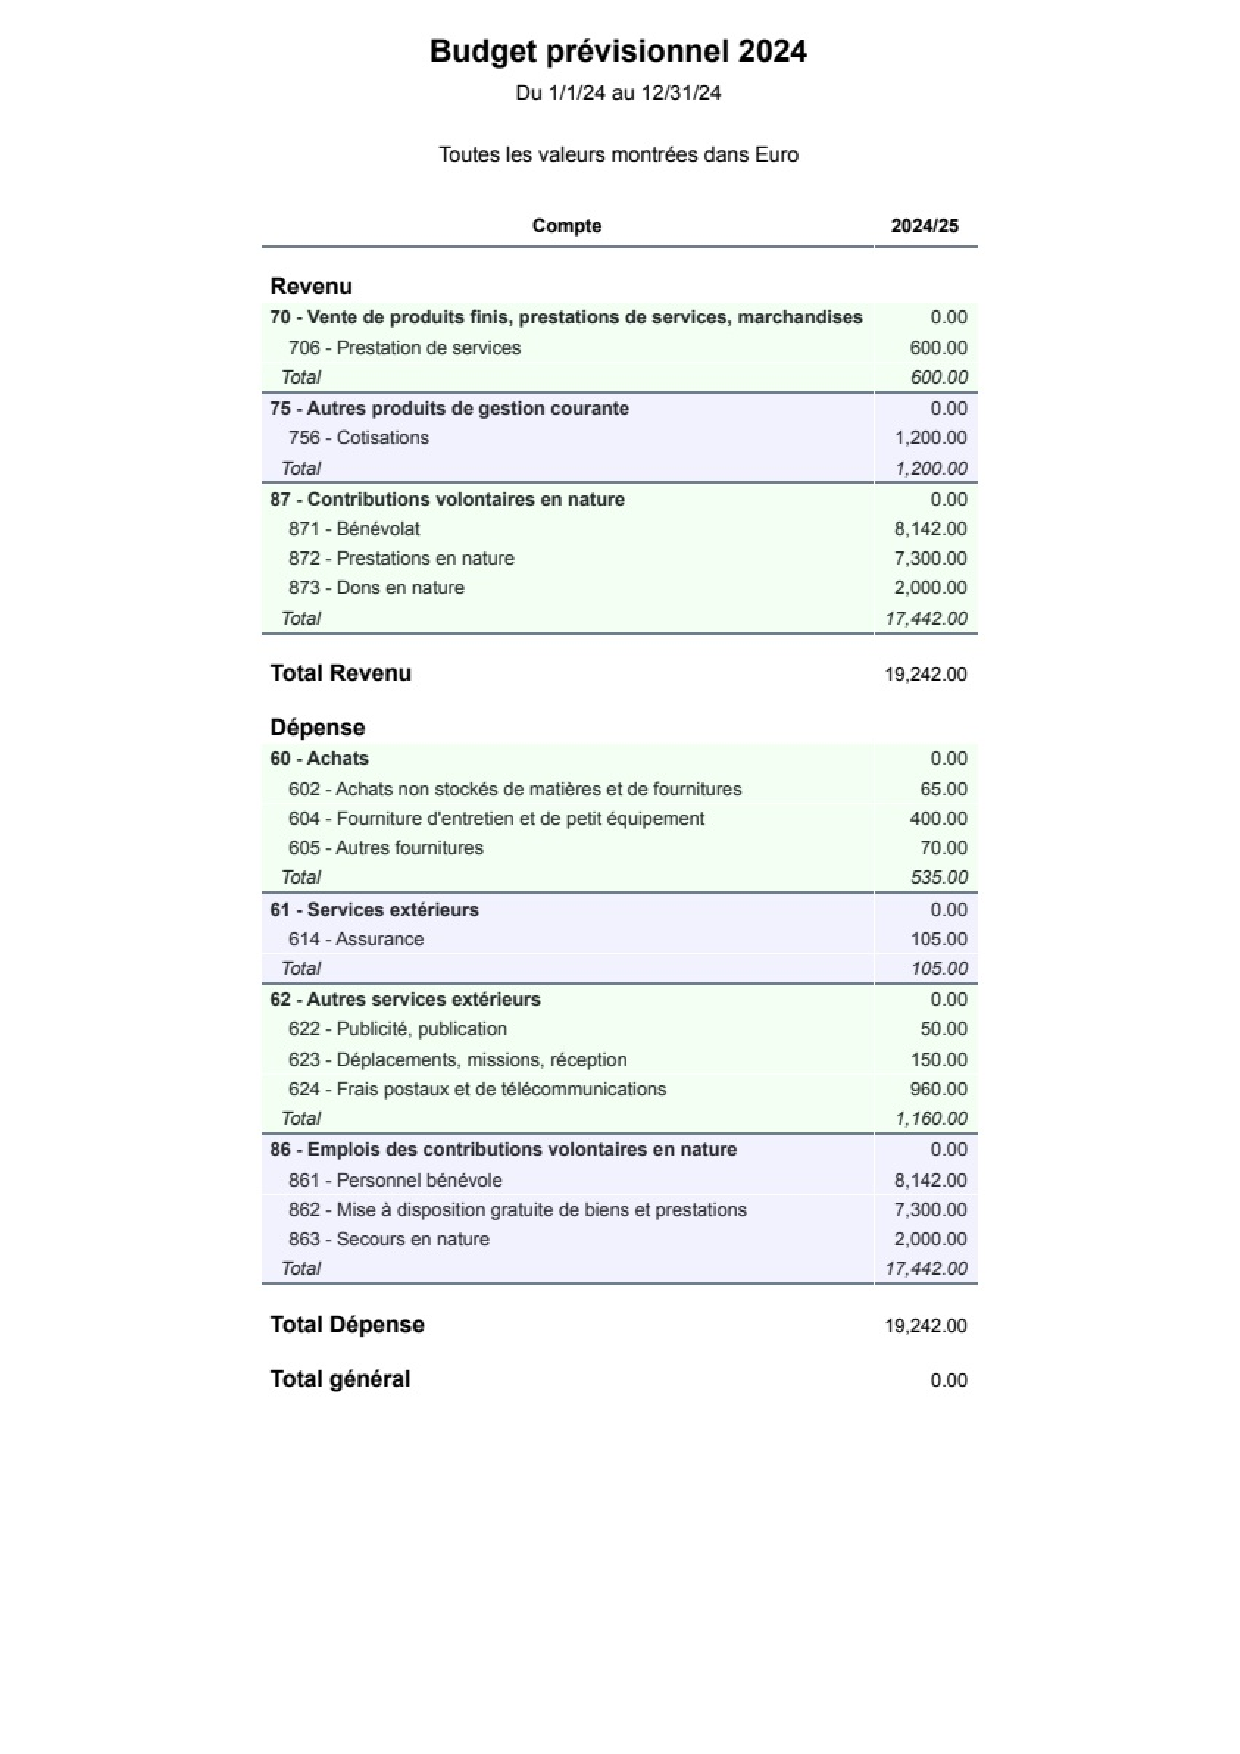
\includepdf[pages=-]{prev2024.pdf}

\section{Questions Diverses}

\newpage

\hrule
\vspace{.3cm}
\begin{center}
\Large\bfseries Assemblée Générale Extraordinaire
\end{center}
\vspace{.3cm}
\hrule

\vspace{1.5cm}

\section*{Déroulement}

\begin{enumerate}
    \item Appel et annonce des procurations
    \item Modification du siège social
	\item Modification des modalité d’organisation des assemblées
\end{enumerate}

\setcounter{section}{1}
\section*{Clotûre}


\end{document}

% vim: set spelllang=fr:

